\documentclass{beamer}
\usepackage{amsmath}
\usepackage{listings}
\usepackage{xcolor}
\usetheme{Madrid} % Added a theme for better visual structure

\title{Stability Analysis of Discrete-Time System}
\author{}
\date{\today}
\lstset{
language=Python,
basicstyle=\ttfamily\small,
keywordstyle=\color{blue},
stringstyle=\color{red},
commentstyle=\color{green!60!black},
numbers=left,
numberstyle=\tiny,
stepnumber=1,
numbersep=8pt,
backgroundcolor=\color{gray!10},
frame=single,
breaklines=true,
showstringspaces=false
}
\begin{document}

\frame{\titlepage}

%------------------------------------------------
\begin{frame}{Problem Statement}
	Consider the discrete-time system shown in the figure where the impulse response $G(z)$ is $g(0)=0$,$g(1)=g(2)=1$, $g(3)=g(4)=...=0$
	\begin{figure}
		\centering
		
\includegraphics[scale=0.5]{figs/question.png}
	\end{figure}
	This system is stable for range of values of $K$
	\begin{enumerate}
		\item $[-1,1/2]$
		\item $[-1, 1]$
		\item $[-1/2,1]$
		\item $[-1/2,2]$
	\end{enumerate}
\end{frame}

%------------------------------------------------
\begin{frame}{Step 1: Impulse Response to Transfer Function}
Impulse response definition:
\[
G(z) = \sum g(n)z^{-n}
\]
Given $g(1)=1$ and $g(2)=1$:
\[
G(z) = z^{-1} + z^{-2}
\]
\begin{block}{Key Idea}
$z^{-1}$ represents a one-step delay in the discrete-time domain.
\end{block}
\end{frame}

%------------------------------------------------
\begin{frame}{Step 2: Block Diagram Equation}
From the feedback loop logic:
\[
Y(z) = G(z)\big(X(z) + K Y(z)\big)
\]
Substitute $G(z)$:
\[
Y(z) = (z^{-1}+z^{-2})(X(z) + K Y(z))
\]
\end{frame}

%------------------------------------------------
\begin{frame}{Step 3: Expand the Equation}
Expand terms:
\[
Y(z) = (z^{-1}+z^{-2})X(z) + K(z^{-1}+z^{-2})Y(z)
\]
Rearrange to group $Y(z)$:
\[
Y(z) - K(z^{-1}+z^{-2})Y(z) = (z^{-1}+z^{-2})X(z)
\]
Factor $Y(z)$:
\[
Y(z)\big[1 - K(z^{-1}+z^{-2})\big] = (z^{-1}+z^{-2})X(z)
\]
\end{frame}

%------------------------------------------------
\begin{frame}{Step 4: Characteristic Equation}
For stability, focus on the denominator of the transfer function $H(z) = \frac{Y(z)}{X(z)}$:
\[
1 - K(z^{-1}+z^{-2}) = 0
\]
Multiply by $z^2$ to get the standard polynomial form:
\[
z^2 - Kz - K = 0
\]
\begin{block}{Characteristic Polynomial}
\[ P(z) = z^2 - Kz - K \]
\end{block}
\end{frame}

%------------------------------------------------
\begin{frame}{Step 5: Stability Concept}
For discrete-time systems:
\begin{block}{Stability Condition}
All roots of the characteristic equation must satisfy:
\[
|z| < 1
\]
\end{block}

Instead of solving for roots directly, we apply the **Jury Stability Test**.
\end{frame}

%------------------------------------------------
\begin{frame}{Jury Stability Test (2nd Order)}
For a second-order polynomial $z^2 + a_1 z + a_0$, the stability conditions are:
\begin{enumerate}
    \item $|a_0| < 1$
    \item $P(1) > 0 \implies 1 + a_1 + a_0 > 0$
    \item $P(-1) > 0 \implies 1 - a_1 + a_0 > 0$
\end{enumerate}
All three must be satisfied for the system to be stable.
\end{frame}

%------------------------------------------------
\begin{frame}{Step 6: Apply Jury Test}
Our polynomial: $z^2 - Kz - K$ \\
Here, $a_1 = -K$ and $a_0 = -K$.

\textbf{Condition 1:} $|-K| < 1 \implies |K| < 1$

\textbf{Condition 2:} $1 + (-K) + (-K) > 0$
\[
1 - 2K > 0 \implies K < \frac{1}{2}
\]

\textbf{Condition 3:} $1 - (-K) + (-K) > 0$
\[
1 > 0 \quad (\text{Always true})
\]
\end{frame}

%------------------------------------------------
\begin{frame}{Final Answer}
Combining the active constraints:
\[
|K| < 1 \quad \text{and} \quad K < \frac{1}{2}
\]
This results in the range:
\[
\boxed{-1 < K < \frac{1}{2}}
\]
\begin{block}{Conclusion}
The system is stable if and only if $K$ stays within this interval.
\end{block}
\end{frame}

%------------------------------------------------
\begin{frame}{Key Takeaways}
\begin{itemize}
    \item $z^{-1}$ functions as a unit delay.
    \item The characteristic equation determines system behavior.
    \item Stability requires poles to stay inside the **Unit Circle**.
    \item The **Jury Test** is a powerful tool for checking stability without calculating complex roots.
\end{itemize}
\end{frame}

\lstinputlisting{codes/verify.py}

\begin{frame}{Input Signal}
\begin{center}
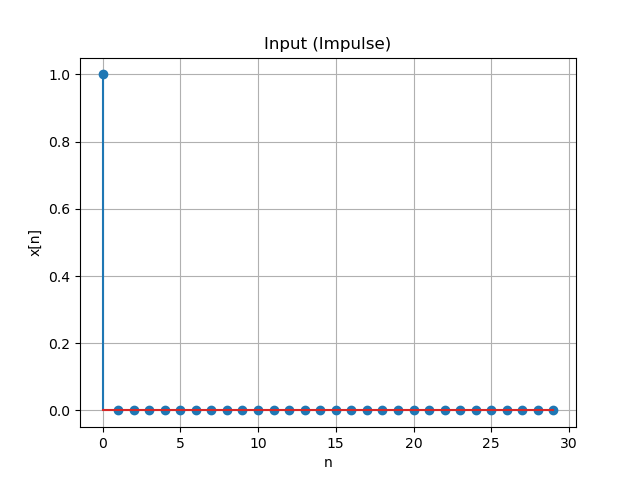
\includegraphics[width=0.8\linewidth]{figs/input.png}
\end{center}
\end{frame}

%---------------------------------------------

\begin{frame}{Impulse Response}
\begin{center}
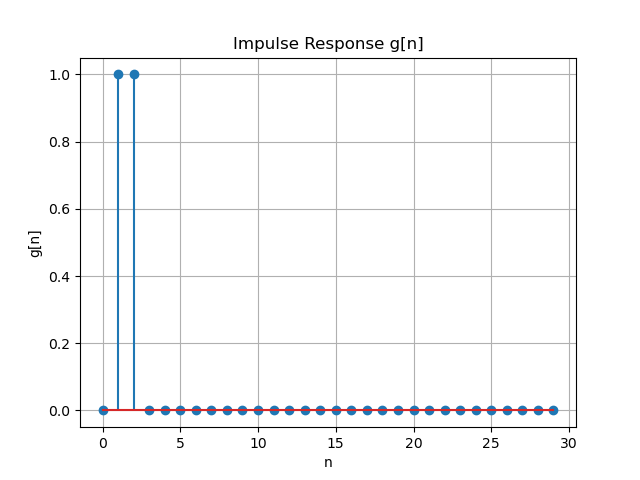
\includegraphics[width=0.8\linewidth]{figs/impulse.png}
\end{center}
\end{frame}

%---------------------------------------------

\begin{frame}{System Output (Stable Case)}
\begin{center}
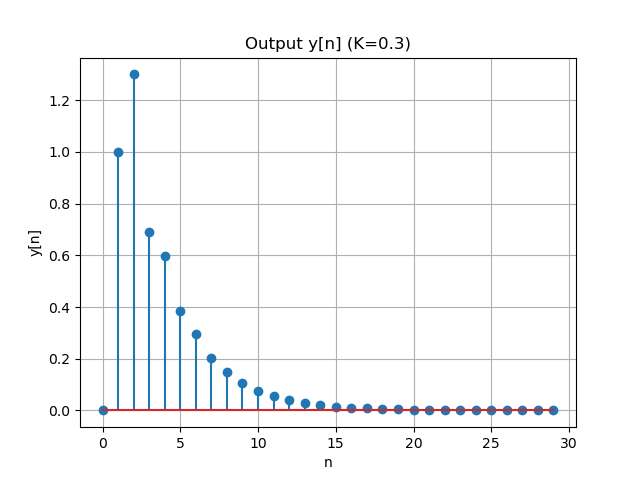
\includegraphics[width=0.8\linewidth]{figs/output.png}
\end{center}

\begin{block}{Observation}
Output decays $\Rightarrow$ system is stable
\end{block}
\end{frame}
\end{document}
